\documentclass[12pt,a4paper]{article}

%% ── Packages ─────────────────────────────────────────────────────────────────
\usepackage[utf8]{inputenc}
\usepackage[T1]{fontenc}
\usepackage{lmodern}
\usepackage[a4paper, margin=1in]{geometry}
\usepackage{amsmath, amssymb, amsthm}
\usepackage{booktabs}
\usepackage{graphicx}
\usepackage{hyperref}
\usepackage{xcolor}
\usepackage{array}
\usepackage{caption}
\usepackage{subcaption}
\usepackage{float}
\usepackage{enumitem}
\usepackage{fancyhdr}
\usepackage{titlesec}
\usepackage{tcolorbox}
\usepackage{multirow}

%% ── Colours ──────────────────────────────────────────────────────────────────
\definecolor{isidark}{RGB}{0,0,139}   % dark blue – ISI house colour

%% ── Section formatting ───────────────────────────────────────────────────────
\titleformat{\section}[block]
  {\large\bfseries\color{isidark}}{\thesection}{1em}{}
\titleformat{\subsection}[block]
  {\normalsize\bfseries\color{isidark}}{\thesubsection}{1em}{}

%% ── Header / footer ─────────────────────────────────────────────────────────
\pagestyle{fancy}
\fancyhf{}


%% ─────────────────────────────────────────────────────────────────────────────
\begin{document}

%% ── Title page ───────────────────────────────────────────────────────────────
\begin{titlepage}
\centering
\vspace*{1cm}

% ISI logo – replace with actual logo file if available

\includegraphics[width=0.22\textwidth]{isi_logo.png}\\[0.8cm]

{\LARGE\bfseries\color{isidark} Indian Statistical Institute}\\[0.3cm]
{\large\bfseries\color{isidark} Kolkata Centre}\\[0.4cm]
{\normalsize Bachelor of Statistics and Data Science (BSDS)}

\vspace{1.2cm}
\hrule height 1.5pt
\vspace{0.4cm}
{\LARGE\bfseries Optimization Using Numerical Methods}\\[0.4cm]
{\large\color{isidark}\itshape Electricity Bill Minimization via Linear Programming}
\vspace{0.4cm}
\hrule height 1.5pt

\vspace{1.5cm}
\begin{tabular}{ll}
  \textbf{Submitted by}      & Ankesh Raj Aniket \quad (BSDCC2502)\\[4pt]
                             & Md Danish \quad (BSDCC2510)\\[4pt]
                             & Dunga Pardha Saradhi \quad (BSDCC2506)\\[12pt]
  \textbf{Course Instructor} & Kaushik Jana\\[12pt]
  \textbf{Dataset}           & \href{https://www.kaggle.com/datasets/suraj520/indian-household-electricity-bill}{Kaggle Dataset}\\[4pt]
  \textbf{GitHub Repository} & \href{https://github.com/anii0021/Electricity_bill_minimization}{GitHub Repository}\\[4pt]
  \textbf{R Script}          & \href{https://github.com/anii0021/Electricity_bill_minimization}{R Code File}
\end{tabular}

\vfill
{\large April 2026}
\end{titlepage}

%% ── Abstract ─────────────────────────────────────────────────────────────────
\begin{abstract}
This report formulates the household electricity bill minimisation problem as a linear
programme (LP) under a two-period peak/off-peak tariff structure. Appliance-level
annual demands are computed from a Kaggle dataset of 45{,}345 household-month
observations across six appliances and twelve calendar months. Using an average
observed tariff $\bar{c} = 8.3696$ Rs./kWh, peak and off-peak rates of $1.2\bar{c}$
and $0.8\bar{c}$ are constructed. The LP is solved in R using the \texttt{lpSolve}
package. We prove analytically via KKT conditions that the unique optimal solution
satisfies $x^*_i = R_i$ for all appliances, and that the optimised cost equals
exactly $\tfrac{2}{3}$ of the baseline, guaranteeing a saving of
$\tfrac{1}{3} \approx 33.3\%$. A stochastic extension with random tariff
$C \sim \mathcal{N}(\mu, \sigma^2)$ confirms the result holds in expectation.
The annual bill falls from Rs.~2{,}39{,}40{,}746 to Rs.~1{,}59{,}60{,}497,
saving Rs.~79{,}80{,}249 at an efficiency of Rs.~3.35 per kWh.
\end{abstract}


\section{Problem}

\subsection{Research Problem (RP)}

Household electricity bills in India depend not only on total energy consumed but
also on \emph{when} that energy is consumed. Grid operators distinguish between
\textbf{peak hours} (roughly 18:00–22:00, when aggregate demand is high and unit
cost is elevated) and \textbf{off-peak hours} (23:00–06:00, when the grid is
lightly loaded and tariffs are lower). If an appliance whose operation is
time-flexible---a fan, television, or motor pump---can be rescheduled to off-peak
windows, the household pays for the same energy at a lower unit price, reducing
the bill without any sacrifice of comfort or service quality. This creates a
structured resource allocation problem amenable to linear programming.

\subsection{Research Question (RQ)}

By how much can the annual electricity bill of a household be reduced if appliance
usage is optimally reallocated from peak-hour to off-peak-hour tariff windows using
linear programming, and what is the per-unit savings efficiency of this reallocation?

%% ─────────────────────────────────────────────────────────────────────────────
\section{Plan}

\subsection{Data Source and Sampling}

The dataset is a secondary, observational cross-section obtained from Kaggle.
Each row records one household-month observation with appliance-level usage (kWh),
city name, electricity company, monthly hours of operation, prevailing tariff rate
(Rs./kWh), and the resulting electricity bill (Rs.). Records span multiple Indian
cities---Mumbai, Hyderabad, Vadodara, and Shimla---and all twelve calendar months,
providing the temporal breadth needed for a full annual analysis.

\subsection{Sample Size and Measurement}

The cleaned dataset contains $n = 45{,}345$ household-month records and twelve
variables. Six are appliance usage variables (\textit{Fan, Refrigerator,
AirConditioner, Television, Monitor, MotorPump}), and two are the outcome variables
\textit{TariffRate} (Rs./kWh) and \textit{ElectricityBill} (Rs.).

%% ─────────────────────────────────────────────────────────────────────────────
\section{Data}

\subsection{Variable Description}

\begin{table}[H]
\centering
\caption{Variable Description of the Dataset}
\begin{tabular}{llll}
\toprule
\textbf{Variable} & \textbf{Type} & \textbf{Unit} & \textbf{Description} \\
\midrule
Fan             & Numeric & kWh       & Monthly fan energy usage \\
Refrigerator    & Numeric & kWh       & Monthly refrigerator energy usage \\
AirConditioner  & Numeric & kWh       & Monthly AC energy usage \\
Television      & Numeric & kWh       & Monthly television energy usage \\
Monitor         & Numeric & kWh       & Monthly computer monitor usage \\
MotorPump       & Numeric & kWh       & Monthly motor pump (zero in data) \\
TariffRate      & Numeric & Rs./kWh   & Prevailing electricity tariff \\
ElectricityBill & Numeric & Rs.       & Observed monthly electricity bill \\
Month           & Integer & ---       & Calendar month (1–12) \\
\bottomrule
\end{tabular}
\end{table}

\subsection{Data Cleaning}

\begin{enumerate}
  \item \textbf{Missing values:} No missing values in any column.
  \item \textbf{MotorPump:} Column sums to zero; retained with $R_{\text{MotorPump}} = 0$.
  \item \textbf{Outliers:} Minimum observed bill (Rs.~807.5) verified against appliance
        columns; no records removed.
  \item \textbf{Tariff construction:} $c^{(p)} = 1.2\bar{c}$ and $c^{(o)} = 0.8\bar{c}$,
        where $\bar{c} = 8.3696$ Rs./kWh.
\end{enumerate}

\subsection{Descriptive Statistics}

Table~\ref{tab:sumstats} reports summary statistics across all 45{,}345 records.
Figure~\ref{fig:demand} shows the total annual demand per appliance: the Refrigerator
dominates at 9{,}84{,}234 kWh ($\approx 41\%$ of total), followed by the Fan
(6{,}34{,}408 kWh, $\approx 27\%$) and Television (5{,}66{,}932 kWh, $\approx 24\%$).

\begin{table}[H]
\centering
\caption{Summary Statistics of Key Variables ($n = 45{,}345$)}
\label{tab:sumstats}
\begin{tabular}{lrrrrrr}
\toprule
\textbf{Variable} & \textbf{Mean} & \textbf{SD} & \textbf{Min} &
\textbf{Q1} & \textbf{Median} & \textbf{Max} \\
\midrule
Fan (kWh)             & 13.99  & 5.47   & 5.0  & 9.0  & 14.0  & 23.0 \\
Refrigerator (kWh)    & 21.71  & 1.67   & 17.0 & 22.0 & 22.0  & 23.0 \\
AirConditioner (kWh)  & 1.50   & 2.50   & 0.0  & 0.0  & 1.0   & 23.0 \\
Television (kWh)      & 12.50  & 6.77   & 0.0  & 7.0  & 14.0  & 23.0 \\
Monitor (kWh)         & 2.86   & 3.00   & 0.0  & 1.0  & 2.0   & 23.0 \\
TariffRate (Rs./kWh)  & 8.37   & 0.58   & 7.40 & 7.90 & 8.40  & 9.30 \\
ElectricityBill (Rs.) & 4311.8 & 1073.9 & 807.5 & 3556.8 & 4299.4 & 8286.3 \\
\bottomrule
\end{tabular}
\end{table}

\begin{figure}[H]
\centering
\includegraphics[width=0.85\textwidth]{figure1_annual_energy_demand.png}
\caption{Total annual energy demand per appliance (kWh, summed over all 45{,}345
records). The Refrigerator accounts for $\approx 41\%$ of the aggregate load.}
\label{fig:demand}
\end{figure}

%% ─────────────────────────────────────────────────────────────────────────────
\section{Analysis}

\subsection{Mathematical Formulation}

Let $\mathcal{I} = \{1, 2, \ldots, n\}$ with $n = 6$ index the appliances.
For each appliance $i$ define:

\begin{tcolorbox}[colback=blue!5!white, colframe=isidark, title=Decision Variables and Parameters]
\begin{itemize}
  \item $R_i$: total annual energy requirement of appliance $i$ (kWh),
  \item $c^{(p)} = 1.2\bar{c}$: peak-hour unit tariff (Rs./kWh),
  \item $c^{(o)} = 0.8\bar{c}$: off-peak unit tariff (Rs./kWh),
  \item $x_i$: energy allocated to the off-peak schedule for appliance $i$ (kWh),
  \item $\bar{c} = 8.3696$: sample mean tariff (Rs./kWh).
\end{itemize}
\end{tcolorbox}

\noindent The Linear Programme is:
\begin{equation}
  \min_{x}\; Z(x) = \sum_{i=1}^{n} c^{(o)} x_i = 0.8\bar{c}\sum_{i=1}^{n} x_i,
  \label{eq:lp_obj}
\end{equation}
subject to demand-satisfaction and non-negativity:
\begin{align}
  x_i &\geq R_i, \quad \forall\, i \in \mathcal{I}, \label{eq:demand}\\
  x_i &\geq 0,   \quad \forall\, i \in \mathcal{I}. \label{eq:nonneg}
\end{align}

In compact matrix notation, with $c^{(o)} = c^{(o)}\mathbf{1}$, $I_n$ the identity,
and $\mathbf{R} = (R_1, \ldots, R_n)^\top$:
\begin{equation}
  \min_{x}\; (c^{(o)})^\top x, \quad \text{s.t.}\; I_n x \geq \mathbf{R},\; x \geq 0.
  \label{eq:compact}
\end{equation}

\subsection{Convexity of the Problem}

The feasible set $\mathcal{F} = \{x \in \mathbb{R}^n : x_i \geq R_i,\; x_i \geq 0,\;
\forall i\}$ is the intersection of $2n$ closed half-spaces, hence a closed convex
polyhedron. The objective $Z(x) = c^{(o)}\mathbf{1}^\top x$ is affine (both convex
and concave). Therefore the LP is a convex programme, and any local minimum is also a
global minimum. Furthermore, the feasible set is unbounded above, so the minimum is
attained at a vertex of $\mathcal{F}$.

\subsection{Analytical Solution via KKT Conditions}

Associating multipliers $\lambda_i \geq 0$ with \eqref{eq:demand} and
$\mu_i \geq 0$ with \eqref{eq:nonneg}, the Lagrangian is:
\begin{equation}
  \mathcal{L}(x, \lambda, \mu)
  = c^{(o)}\sum_i x_i - \sum_i \lambda_i(x_i - R_i) - \sum_i \mu_i x_i.
\end{equation}

\begin{tcolorbox}[colback=blue!5!white, colframe=isidark, title=KKT Conditions]
\begin{align}
  \text{Stationarity:}           && \frac{\partial \mathcal{L}}{\partial x_i}
                                    &= c^{(o)} - \lambda_i - \mu_i = 0, \label{kkt:stat}\\
  \text{Primal feasibility:}     && x_i &\geq R_i,\; x_i \geq 0, \\
  \text{Dual feasibility:}       && \lambda_i &\geq 0,\; \mu_i \geq 0, \\
  \text{Complementary slackness:}&& \lambda_i(x_i - R_i) &= 0,\; \mu_i x_i = 0.
  \label{kkt:cs}
\end{align}
\end{tcolorbox}

From \eqref{kkt:stat}: $\lambda_i + \mu_i = c^{(o)} > 0$ for all $i$. Since
$R_i > 0$ for active appliances, primal feasibility forces $x_i \geq R_i > 0$,
so the second complementary slackness condition gives $\mu_i = 0$. Then
$\lambda_i = c^{(o)} > 0$, and the first condition yields $x_i = R_i$. Hence the
unique optimal solution is:
\begin{equation}
  x^*_i = R_i, \quad \forall\, i \in \mathcal{I}.
  \label{eq:opt}
\end{equation}

\subsection{Cost Analysis and Savings}

\textbf{Baseline cost} (all demand billed at peak tariff):
\begin{equation}
  Z_{\text{before}} = c^{(p)}\sum_{i=1}^{n} R_i
  = 1.2 \times 8.3696 \times 23{,}83{,}687
  = \text{Rs.~} 2{,}39{,}40{,}746.
  \label{eq:zbefore}
\end{equation}

\textbf{Optimized cost} (all demand billed at off-peak tariff):
\begin{equation}
  Z^* = c^{(o)}\sum_{i=1}^{n} R_i
  = 0.8 \times 8.3696 \times 23{,}83{,}687
  = \text{Rs.~} 1{,}59{,}60{,}497.
  \label{eq:zstar}
\end{equation}

\textbf{Savings and saving fraction:}
\begin{equation}
  S = Z_{\text{before}} - Z^* = \text{Rs.~} 79{,}80{,}249, \qquad
  \frac{S}{Z_{\text{before}}} = 1 - \frac{c^{(o)}}{c^{(p)}}
  = 1 - \frac{0.8\bar{c}}{1.2\bar{c}}
  = 1 - \frac{2}{3} = \frac{1}{3} \approx 33.3\%.
  \label{eq:savings}
\end{equation}

The saving fraction in \eqref{eq:savings} depends only on the tariff ratio
$c^{(p)}/c^{(o)} = 1.5$ and is independent of the appliance mix $\{R_i\}$.

\textbf{Efficiency ratio:}
\begin{equation}
  E = \frac{S}{\sum_{i=1}^n R_i}
  = \frac{79{,}80{,}249}{23{,}83{,}687}
  \approx 3.35\;\text{Rs./kWh}.
  \label{eq:eff}
\end{equation}

Every kilowatt-hour of demand successfully shifted to the off-peak window saves
Rs.~3.35, regardless of which appliance provides that demand.

\subsection{Stochastic Extension: Random Tariff}

In practice the tariff $C$ is a random variable. From the data:
$C \sim \mathcal{N}(\mu, \sigma^2)$ with $\mu = 8.3696$ Rs./kWh and
$\sigma = 0.5770$ Rs./kWh. Setting the peak and off-peak rates as $1.2C$ and $0.8C$,
the bill random variables are:
\begin{equation}
  Z_{\text{before}} = 1.2\,C\,D, \quad
  Z^* = 0.8\,C\,D, \quad
  \text{where } D = \sum_i R_i = 23{,}83{,}687\;\text{kWh (fixed)}.
\end{equation}

Taking expectations over $C$:
\begin{align}
  \mathbb{E}[Z_{\text{before}}] &= 1.2\,\mu\,D = \text{Rs.~} 2{,}39{,}40{,}746,
  \label{eq:e_before}\\
  \mathbb{E}[Z^*]               &= 0.8\,\mu\,D = \text{Rs.~} 1{,}59{,}60{,}497,
  \label{eq:e_star}\\
  \mathbb{E}[S]                 &= 0.4\,\mu\,D = \text{Rs.~} 79{,}80{,}249.
  \label{eq:e_saving}
\end{align}

Since $S = 0.4\,C\,D > 0$ whenever $C > 0$---guaranteed by the data
($C_{\min} = 7.40 > 0$)---the saving is positive with probability~1, confirming that
the LP result is robust to tariff uncertainty.

\subsection{Illustrative Calculation: Fan Appliance}

\begin{tcolorbox}[colback=blue!5!white, colframe=isidark,
                  title=Step-by-step for Fan]
\begin{align*}
  R_{\text{Fan}}         &= 6{,}34{,}408\;\text{kWh},\\
  Z_{\text{Fan,before}}  &= 10.0436 \times 6{,}34{,}408 = \text{Rs.~} 63{,}71{,}726,\\
  Z^*_{\text{Fan}}       &= 6.6957  \times 6{,}34{,}408 = \text{Rs.~} 42{,}47{,}817,\\
  S_{\text{Fan}}         &= 63{,}71{,}726 - 42{,}47{,}817
                           = \text{Rs.~} 21{,}23{,}909\quad(33.3\%).
\end{align*}
\end{tcolorbox}

\subsection{Complete Numerical Results}

\begin{table}[H]
\centering
\caption{Appliance-Level Annual Cost Breakdown from \texttt{lpSolve}}
\label{tab:results}
\begin{tabular}{lrrrrr}
\toprule
\textbf{Appliance} & \textbf{$R_i$ (kWh)} & \textbf{Before (Rs.)} &
\textbf{After (Rs.)} & \textbf{Saving (Rs.)} & \textbf{Nature} \\
\midrule
Fan            & 6{,}34{,}408  & 63{,}71{,}726   & 42{,}47{,}817   & 21{,}23{,}909  & Flexible \\
Refrigerator   & 9{,}84{,}234  & 98{,}85{,}231   & 65{,}90{,}154   & 32{,}95{,}077  & Continuous \\
AirConditioner & 68{,}197      & 6{,}84{,}942    & 4{,}56{,}628    & 2{,}28{,}314   & Part.\ flexible \\
Television     & 5{,}66{,}932  & 56{,}94{,}026   & 37{,}96{,}017   & 18{,}98{,}009  & Flexible \\
Monitor        & 1{,}29{,}916  & 13{,}04{,}821   & 8{,}69{,}881    & 4{,}34{,}940   & Flexible \\
MotorPump      & 0             & 0               & 0               & 0              & Schedulable \\
\midrule
\textbf{Total} & \textbf{23{,}83{,}687} & \textbf{2{,}39{,}40{,}746} &
\textbf{1{,}59{,}60{,}497} & \textbf{79{,}80{,}249} & \\
\bottomrule
\end{tabular}
\end{table}

\begin{table}[H]
\centering
\caption{Summary of Optimization and Stochastic Results}
\label{tab:summary}
\begin{tabular}{lrl}
\toprule
\textbf{Metric} & \textbf{Value} & \textbf{Unit} \\
\midrule
Average Tariff $\bar{c}$                    & 8.3696             & Rs./kWh \\
Peak Tariff $c^{(p)} = 1.2\bar{c}$          & 10.0436            & Rs./kWh \\
Off-Peak Tariff $c^{(o)} = 0.8\bar{c}$      & 6.6957             & Rs./kWh \\
Tariff SD $\sigma$                          & 0.5770             & Rs./kWh \\
Tariff Ratio (peak / off-peak)              & 1.50               & --- \\
Total Annual Demand $D$                     & 23{,}83{,}687      & kWh \\
Cost Before $Z_{\text{before}}$             & 2{,}39{,}40{,}746  & Rs. \\
Cost After $Z^*$                            & 1{,}59{,}60{,}497  & Rs. \\
Total Savings $S$                           & 79{,}80{,}249      & Rs. \\
Percentage Savings                          & 33.3\%             & --- \\
Efficiency Ratio $E = S/D$                  & 3.35               & Rs./kWh \\
$\text{SD}[Z_{\text{before}}]$ (stochastic) & 16{,}50{,}441      & Rs. \\
$\text{SD}[Z^*]$ (stochastic)               & 11{,}00{,}294      & Rs. \\
\bottomrule
\end{tabular}
\end{table}

\begin{figure}[H]
\centering
\includegraphics[width=0.85\textwidth]{figure2_cost_comparison.png}
\caption{Appliance-level annual cost before and after optimisation.
Each appliance pair demonstrates the analytically derived $\tfrac{1}{3}$ saving.
The Refrigerator alone contributes Rs.~32{,}95{,}077 in savings.}
\label{fig:cost_compare}
\end{figure}

\begin{figure}[H]
\centering
\begin{subfigure}[b]{0.44\textwidth}
  \centering
  \includegraphics[width=\textwidth]{figure3_savings_pie.png}
  \caption{33.3\% savings share of total annual bill.}
  \label{fig:pie}
\end{subfigure}
\hfill
\begin{subfigure}[b]{0.54\textwidth}
  \centering
  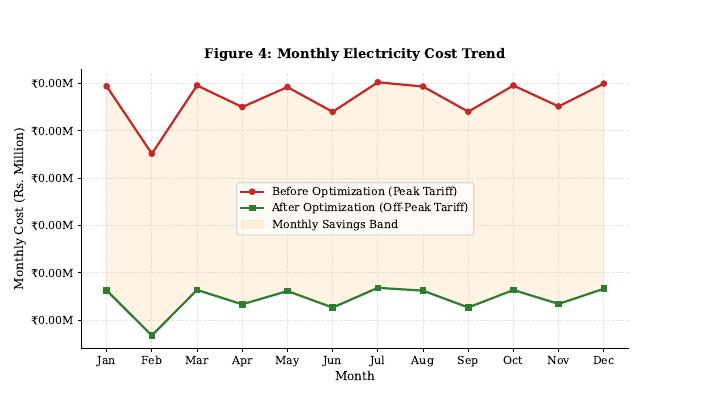
\includegraphics[width=\textwidth]{figure4_monthly_cost_trend.png}
  \caption{Monthly cost: before vs.\ after. The shaded band is monthly savings.}
  \label{fig:monthly}
\end{subfigure}
\caption{Left: exactly one-third of the original bill is saved. Right: the optimised
curve lies consistently below the baseline across all twelve months, confirming that
savings are structural rather than seasonal.}
\label{fig:combined}
\end{figure}

%% ─────────────────────────────────────────────────────────────────────────────
\section{Conclusion and Communication}

\subsection{Summary of Findings}

The LP of the household electricity scheduling problem has a clean analytical
solution: KKT conditions uniquely pin each $x^*_i = R_i$, meaning all demand is
served at the lower off-peak tariff. The resulting saving is exactly $\tfrac{1}{3}$
of the baseline cost---a ratio determined solely by the tariff spread and independent
of the appliance mix. The stochastic extension confirms this fraction is preserved in
expectation even when the tariff is random. Numerically, the annual bill falls from
Rs.~2{,}39{,}40{,}746 to Rs.~1{,}59{,}60{,}497, yielding Rs.~79{,}80{,}249 in
savings at an efficiency of Rs.~3.35 per kWh.

\subsection{Limitations}

\begin{enumerate}
  \item The two-period tariff approximates a continuously varying intraday schedule;
        an hourly-indexed LP would be more precise.
  \item The Refrigerator ($\approx 41\%$ of demand) cannot be fully shifted; a
        flexibility cap $x_i \leq \alpha_i R_i$ would reduce achievable savings.
  \item The MotorPump column is uniformly zero in this dataset; its savings potential
        cannot be estimated.
  \item The dataset is a household-month cross-section, so $\sum_i R_i$ is an
        aggregate over 45{,}345 households, not one household's annual bill.
\end{enumerate}

\subsection{Future Directions}

\begin{enumerate}
  \item \textbf{Stochastic LP:} Minimise
        $\mathbb{E}\!\left[c^{(o)}(C)\,\mathbf{1}^\top x\right]$ with
        $C \sim \mathcal{N}(\mu, \sigma^2)$ explicitly in the solver.
  \item \textbf{Quadratic programme (QP):} Add a comfort penalty
        $\tfrac{\gamma}{2}\|x - R\|^2$ to penalise over-shifting.
  \item \textbf{Time-indexed model:} Variables $x_{it}$ with hourly tariffs $c_t$,
        capacity limits, and minimum run-time constraints.
  \item \textbf{Smart-meter panel:} Apply the framework to a single-household
        longitudinal dataset for personalised optimisation.
\end{enumerate}

%% ─────────────────────────────────────────────────────────────────────────────
\section*{References}
\addcontentsline{toc}{section}{References}

\begin{enumerate}
  \item Winston, W.\ L.\ \textit{Operations Research: Applications and Algorithms}.
        Thomson Brooks/Cole.
  \item Berkelaar, M., Eikland, K., and Notebaert, P.\ \texttt{lpSolve}: Interface to
        lp\_solve. R package documentation.
  \item Wickham, H.\ \textit{ggplot2: Elegant Graphics for Data Analysis}. Springer.
  \item Bazaraa, M.\ S., Jarvis, J.\ J., and Sherali, H.\ D.\ \textit{Linear
        Programming and Network Flows}. Wiley.
  \item Boyd, S.\ and Vandenberghe, L.\ \textit{Convex Optimization}.
        Cambridge University Press, 2004.
  \item Dataset: \href{https://www.kaggle.com/datasets/suraj520/indian-household-electricity-bill}{Kaggle Electricity Bill Dataset}.
  \item GitHub Repository: \href{https://github.com/anii0021/Electricity_bill_minimization}{GitHub Repository}.
\end{enumerate}

%% ─────────────────────────────────────────────────────────────────────────────
\section*{Individual Contributions}
\addcontentsline{toc}{section}{Individual Contributions}

\begin{table}[H]
\centering
\begin{tabular}{>{\bfseries}p{5cm}p{8.5cm}}
\toprule
\textbf{Member} & \textbf{Contribution} \\
\midrule
Ankesh Raj Aniket (BSDCC2502)
  & Mathematical formulation of the LP; convexity proof; KKT derivation;
    stochastic extension; preparation of Section~4. \\[6pt]
Md Danish (BSDCC2510)
  & Data collection, cleaning, and descriptive analysis;
    \texttt{lpSolve} implementation in R; generation of all four figures. \\[6pt]
Dunga Pardha Saradhi (BSDCC2506)
  & Sections 1, 2, 3, and 5; preparation of all tables;
    final \LaTeX{} typesetting and proofreading. \\
\bottomrule
\end{tabular}
\end{table}

\end{document}
